\chapter{Preliminares} % (fold)
En  este  capítulo  se hablará  sobre  el  correo  electrónico  y  algunos  de  los intermediarios que hacen posible que este servicio sea usado en toda la red de  internet, también  se describirán las  amenazas a  las  que  se   enfrenta  este  servicio para  hacer  llegar  información  de  un  usuario  a  otro  de  una  manera  segura  y  cuales  han 
sido   las   respuestas   de   los   proveedores   de   servicio   de   correo   electrónico   para proporcionar dicha seguridad a los usuarios. 

\section{Criptografía}


El objetivo fundamental de la criptografía~\cite{stinson} es garantizar que dos entidades, 
usualmente representadas por Alicia y Bob, se comuniquen a trav\'es de un canal inseguro de tal manera que un oponente conocido como \'Oscar, no pueda entender lo que se dice. A dicho oponente se le conoce tambi\'en como
{\it adversario}.
Cuando Alicia manda un mensaje a Bob tambi\'en conocido como {\it texto en claro}, si Oscar intercepta el mensaje puede leer su contenido sin problemas, pero si Alicia cifra el texto en claro usando una clave, ella obtiene un texto cifrado el cual es enviado por el canal de comunicación a Bob. Si Oscar intercepta este mensaje ya no podr\'a leerlo porque no sabe como pasar del texto cifrado al texto el claro, pero Bob si ser\'a capaz de recuperar el texto en claro, por que él sí conoce la clave de cifrado.

Formalmente la criptografía \cite{cri} es el estudio de técnicas matemáticas relacionadas con la seguridad para proveer los
siguientes servicios:
\begin{itemize}
 \item \textbf{Confidencialidad}:  La  información  sólo es  accesible  sólo  para  aquéllos  que  están autorizados.
 \item \textbf{Integridad}:  La información sólo puede ser creada y modificada por quien esté autorizado a hacerlo.
 \item \textbf{Autenticación}: Se garantiza que el mensaje provino del aparente autor o fuente.
 \item \textbf{No repudio}:  Este servicio evita que las entidades en una conexión nieguen compromisos establecidos previamente.
\end{itemize}

Estas técnicas están destinadas a alterar las representaciones lingüísticas de ciertos mensajes con el fin de hacerlos ininteligibles a receptores no autorizados.


\subsection{Tipos de Ataques}
A continuaci\'on se describen   los  tipos de  ataque a  las comunicaciones, los cuales dependen  de 
cuanta  información  tenga  disponible  el  adversario  para  poder  romper  el  cifrado~\cite{at}.
\begin{itemize}
 \item \textbf{Ataque con sólo texto cifrado(Ciphertext-only  attack)}: En este tipo de ataque el adversario tiene acceso sólo al texto cifrado, y no tiene acceso al texto plano, pero es el ataque más débil debido a la falta de información.
 \item \textbf{Ataque de texto plano(Known plaintext attack)}: En este tipo de ataque el adversario se supone que tienen acceso a la lista en un número limitado de pares de texto plano y el texto cifrado correspondiente.
 \item \textbf{Ataque de texto cifrado elegido(Chosen ciphertext attack)}: Este ataque se puede elegir los textos cifrados arbitrariamente y tener acceso a texto planos después de ser procesados. Para que este ataque se lleve a cabo es necesario tener el extremo receptor de la comunicación y acceso al canal de la comunicación.
 \item \textbf{Ataque de texto plano elegido(Chosen plaintext attack)}: Este ataque es capaz de elegir una serie de textos planos para ser cifrados y tener acceso al texto cifrado resultante. Esto le permite explorar cualquier área del espacio de  texto plano que desea y puede permitirle explotar el comportamiento no aleatorio que sólo aparecen con ciertos textos planos.
\end{itemize}
\begin{definition}
Un sistema criptográfico es una quintupla $(\cal M,C,K,E,D)$ donde:

\begin{enumerate}
 \item $\cal M$ es el espacio finito de posibles mensajes en claro.
 \item $\cal C$ es el espacio finito de posibles mensajes cifrados.
 \item $\cal K$ es el espacio finito de posibles claves a utilizar.
 \item Para cada $K \in \cal K$, se tiene una regla $e_k\in \cal{E}$ y su correspondiente regla $d_k\in {\cal D}$. Donde $e_k :\cal M\rightarrow C$ y $d_k:\cal C\rightarrow M$ siendo funciones tales que $d_k(e_k(x))=x$ siendo $x$ un elemento del espacio de textos en claro $x\in\cal M$
\end{enumerate}
\end{definition}


\subsection{Cifrado Simétrico}
Un sistema de cifrado simétrico~\cite{sime} es un tipo de cifrado que usa una misma clave para cifrar y para descifrar. Las dos partes que se comunican mediante el cifrado simétrico deben estar de acuerdo en la clave a usar de antemano. Una vez de acuerdo, el remitente cifra un mensaje usando la clave, lo envía al destinatario, y éste lo descifra usando la misma clave, esto se ilustra en la Figura~\ref{fig:1-2-1}.

\begin{figure}[H]
\centering
	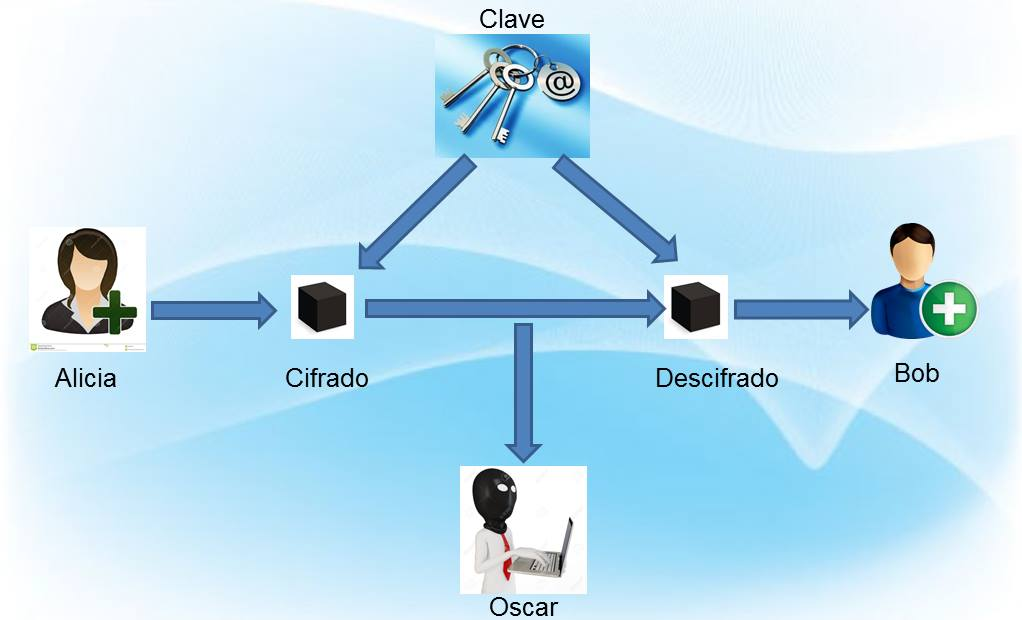
\includegraphics[width=10cm, height=5cm]{./images/simetrico.jpg}
	\caption{Diagrama cifrado simétrico}
	\label{fig:1-2-1}
\end{figure}
La sintaxis de un esquema de cifrado sim\'etrico, esta dada por la siguiente definic\'on.
\begin{definition} 
Un esquema de cifrado sim\'etrico est\'a conformado por una tripleta de algoritmos 
$\sf \Pi=(Gen, Enc, Dec)$, definidos como se describe a continuaci\'on:
\begin{itemize}
\item  El algoritmo generador de claves $\sf Gen$ selecciona una llave  $K$ al azar del conjunto de llaves $\cal K$, esto se denotar\'a como $K \rand {\cal K}$.
Esta clave $K$  ser\'a usada por los algoritmos  $\sf Enc$ y $\sf Dec$, esta clave la compartir\'an  emisor y receptor. 
\item El algoritmo de cifrado $\sf Enc$, toma como entrada un texto en claro  $M \in {\cal M}$ y una clave $K$ generada por  $\sf Gen$  y regresa un texto cifrado $C \in {\cal C}$.  Usualmente esto se denota como $C \leftarrow {\sf Enc}_K(M)$.
 \item El algoritmo de descifrado $\sf Dec$, toma como entrada un texto cifrado $C$ y una llave $K$ y regresa $M$. Esta operaci\'on se denota por  $M \leftarrow {\sf Dec}_K(C)$.
Para que cualquier algoritmo de cifrado sim\'etrico funcione correctamente, se debe garantizar que para
todas las llaves posibles en  $\cal K$ y todos los posibles mensajes $\cal M$, $$ {\sf Dec}_K({\sf Enc}_K(M)) = M.$$
\end{itemize}
\end{definition}

\subsection{Cifrado por bloques}
Este tipo de cifrado toma bloques de información del texto plano y produce bloques de información cifrados de un tamaño fijo, normalmente es del mismo tamaño que el bloque de información del texto plano. Los bloques de cifrado tienen que cumplir la condición de ser lo suficientemente grandes como para evitar ataques de texto cifrado, otra condición que se debe cumplir es que la asignación de bloques de entrada a bloques de salida es uno a uno para hacer el proceso reversible.\\
Formalmente un cifrado en bloque se considera que es seguro si se comporta como una permutación pseudoaleatoria fuerte, es decir, un cifrado de bloques es seguro si un adversario no puede distinguir su salida de una permutación elegida al azar.\\
Para hacer la asignación de bloques los algoritmos de cifrado utilizan sustituciones y permutaciones en los bloques de texto plano hasta obtener un texto cifrado.\\
La sustitución es el reemplazo de un bloque de $n$ bits por otro bloque de $n$ bits en un espacio de 
$2^{k}$~\cite{bloc}. Los cifradores por bloques mas usados son AES (Advanced Encryption Standard, por sus 
siglas en ingl\'es) y DES (Data Encryption Standard, por sus siglas en ingl\'es).



\subsection{Modos de operación}
Los modos de operaci\'on fueron desarrollados para el algoritmo DES, estos fueron estandarizados en Diciembre de 1980. 
Cuando la informaci\'on es cifrada usando la misma clave, surge una serie de problemas de seguridad. En esencia los modos de operaci\'on son una técnica para mejorar el efecto criptogr\'afico de los 
cifradores por bloques~\cite{modes}.\\\\
\textit{ECB}(Electronic codebook): Este modo de operación es probablemente el más simple de todos, el texto plano M está segmentado como $ M=M_1||M_2||...||M_m$ donde cada $M_i$ es un bloque de n bits. A continuación la funci\'on de cifrado $E_k$ se aplica por separado a cada bloque $M_i$. \\
A continuación tenemos el diagrama de este modo de cifrado.\\
\begin{figure}[h]
    \centering
    \begin{subfigure}[t]{0.5\textwidth}
        \centering
        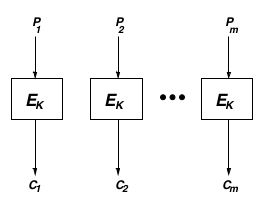
\includegraphics[height=1.7in]{./images/ecb1.png}
        \caption{Diagrama ECB Cifrado}
        \label{fig:1-3-1}
    \end{subfigure}%
    ~ 
    \begin{subfigure}[t]{0.5\textwidth}
        \centering
        \includegraphics[height=1.7in]{./images/ECB2.png}
        \caption{Diagrama ECB Descifrado}
        \label{fig:1-3-1}
    \end{subfigure}
    \label{fig:protocol}
\end{figure}


\textit{CBC}(Cipher-block chaining): Para este modo de operación la salida de un bloque de cifrado se introduce en el siguiente bloque de cifrado junto con el siguiente bloque del mensaje.\\

\begin{figure}[h]
    \centering
    \begin{subfigure}[t]{0.5\textwidth}
        \centering
        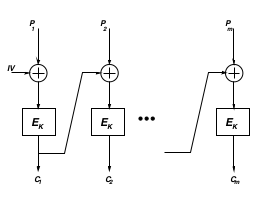
\includegraphics[height=1.7in]{./images/cbc1.png}
        \caption{Diagrama CBC Cifrado}
        \label{fig:1-4-1}
    \end{subfigure}%
    ~ 
    \begin{subfigure}[t]{0.5\textwidth}
        \centering
        \includegraphics[height=1.7in]{./images/CBC2.png}
        \caption{Diagrama CBC Descifrado}
        \label{fig:1-4-1}
    \end{subfigure}
    \label{fig:protocol}
\end{figure}

 \begin{figure}[H]
 \centering
	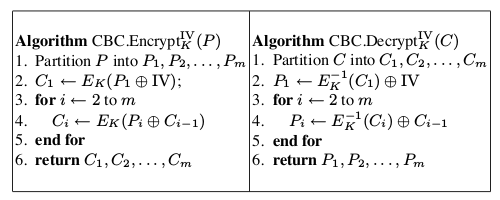
\includegraphics[width=14cm, height=6cm]{./images/pcbc.png}
	
\end{figure}

CBC toma como bloques de mensajes de entrada M y un vector de inicialización (IV). Durante el cifrado, la salida del i-ésimo bloque depende de los i-1 bloques anteriores. Así, el cifrado CBC es intrínsecamente secuencial.\\

\textit{CFB}(Cipher Feedback): En este modo de operación, los bloques de cifrado también están encadenados pero a la salida se produce de una manera muy diferente de la de CBC. Cada bloque de salida se le aplica XOR con el siguiente bloque de entrada.\\

\begin{figure}[h]
    \centering
    \begin{subfigure}[t]{0.5\textwidth}
        \centering
        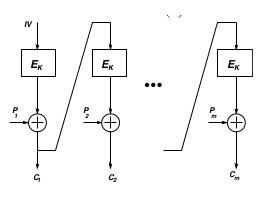
\includegraphics[height=1.7in]{./images/cfb1.png}
		\caption{Diagrama CFB Cifrado}
		\label{fig:1-5-1}
    \end{subfigure}%
    ~ 
    \begin{subfigure}[t]{0.5\textwidth}
        \centering
        \includegraphics[height=1.7in]{./images/CFB2.png}
		\caption{Diagrama CFB Descifrado}
		\label{fig:1-5-1}
    \end{subfigure}
    \label{fig:protocol}
\end{figure}

\begin{figure}[H]
\centering
	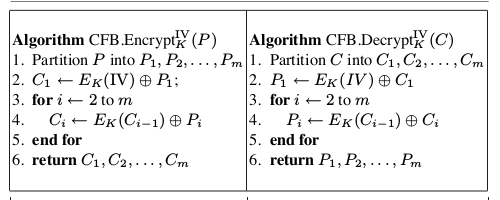
\includegraphics[width=14cm, height=6cm]{./images/pcfb.png}
	
\end{figure}


\textit{OFB}(Output feedback): En este modo de operación el IV se cifra varias veces para obtener un flujo de bytes aleatorios, el resultado de esto se aplica XOR con el bloque de texto plano mientras que el flujo de bytes aleatorios se usa como parámetro del siguiente bloque. A diferencia de los otros modos en OFB ninguna parte del texto claro entra directamente a cifrarse.

\begin{figure}[h]
    \centering
    \begin{subfigure}[t]{0.5\textwidth}
        \centering
        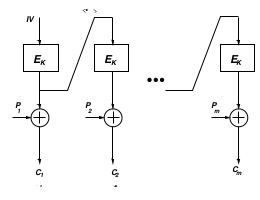
\includegraphics[height=1.7in]{./images/ofb1.png}
		\caption{Diagrama OFB Cifrado}
		\label{fig:1-6-1}
    \end{subfigure}%
    ~ 
    \begin{subfigure}[t]{0.5\textwidth}
        \centering
        \includegraphics[height=1.7in]{./images/OFB2.png}
		\caption{Diagrama OFB Descifrado}
		\label{fig:1-6-1}
    \end{subfigure}
    \label{fig:protocol}
\end{figure}

\begin{figure}[H]
\centering
	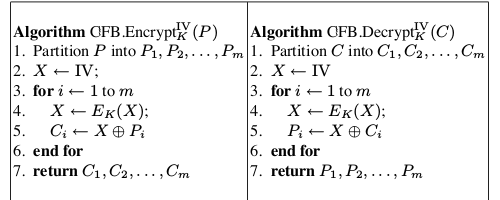
\includegraphics[width=14cm, height=6cm]{./images/pofb.png}
	
\end{figure}
\pagebreak
\subsection{Funciones Hash}
A continuaci\'on se describir\'an las caracter\'isticas de las {\it funciones
hash}, tambi\'en conocidas como {\it funciones de resumen}. Las funciones hash basan
su definici\'on en funciones de un solo sentido  ({\it one-way functions}, en ingl\'es).
Una funci\'on de un s\'olo sentido es aquella que para un valor $x$, es 
muy f\'acil calcular $f(x)$, pero es muy dif\'icil hallar $f^{-1}(x)$. Es 
complicado en general, hallar funciones de \'este tipo y probar que lo 
son.
\begin{definition}
Una funci\'on hash, es una funci\'on de un s\'olo sentidocuya entrada $m$
 es un mensaje de longitud arbitraria
y la salida es una cadena binaria de longitud fija. Al resumen o hash de 
un mensaje $m$, se le denotar\'a como $h(m)$. Una funci\'on hash debe
tener las siguientes propiedades:
\begin{itemize}
\item Para cualquier mensaje $m$, debe ser posible calcular $h(m)$ 
eficientemente. 
\item Dado $h(m)$, debe ser computacionalmente dif\'icil, hallar un mensaje
$m'$, tal que $h(m)=h(m')$.
\item Debe ser computacionalmente dif\'icil, hallar dos mensajes $m$ y $m'$ 
tales que $h(m)=h(m')$.
\end{itemize}
\end{definition}
 
Entre las funciones hash que se usan para criptograf\'ia est\'an: MD2, MD4,
MD5, donde MD significa {\it Message Digest}, y el algoritmo est\'andar al momento de escribir \'estas notas es el {\it Secure Hash Algorithm} por sus siglas
en ingl\'es SHA.
  La MD5 fue dise\~nada por Ron Rivest, toma como entrada un mensaje de 
longitud arbitraria y proporciona como salida una cadena binaria de 128 bits.
El mensaje de entrada se procesa por bloques de 512 bits. 
  La SHA fue dise\~nada por en NIST y se estableci\'o como est\'andar
en 1993. Recibe como entrada un mensaje con longitud menor a $2^{64}$ bits y
como salida se obtiene una cadena binaria de 160 bits. Al igual que el
MD5, se procesa en bloques de 512 bits~\cite{modes}.



%Las funciones hash son usadas para construir una pequeña huella digital de la informaci\'on, si la informaci\'on es alterada tambi\'en la huella digital es alterada. Esta caracter\'istica hace que las funciones hash sean ampliamente usadas para verificar la integridad de datos.\\
%De manera formal, un funci\'on Hash es una Cuadrupla$(X,Y,K,H)$ donde:
%\begin{enumerate}
% \item $X$ es un conjunto de posibles mensajes.
% \item $Y$ es un conjunto finito de posibles resúmenes de mensajes o etiquetas de autenticación.
% \item $K$, el espacio de claves, es un conjunto finito de posibles claves.
% \item Para cada $k\quad \epsilon\quad K$, existe una función hash $h_k\quad \epsilon\quad H$. Parac ada $h_k: X \longrightarrow Y$.
% \cite{stinson}
%\end{enumerate}



\section{Aritmética Modular}
En criptograf\'ia a menudo se recurre a conceptos matem\'aticos del \'area de \'algebra y teor\'ia de n\'umeros, para
construir diversos esquemas criptogr\'aficos. En esta secci\'on se describir\'an los conceptos matem\'aticos,
necesarios para comprender los esquema de cifrado, que se utilizaron en el desarrollo de este trabajo terminal. 

\begin{definition}
Una {\it relaci\'on de congruencia}, denotada por el s\'imbolo $\equiv$, se 
define como sigue: dados dos n\'umeros enteros, $a,b \in \mathbb{Z}$ se dice que son congruentes
m\'odulo $n$, si y solo si $n$ divide a $a-b$, dicho de otra manera si y s\'olo
si $a-b=nq, q \in \mathbb{Z}$. Si $a$ y $b$ son congruentes m\'odulo $n$ se denota como $a \equiv b \bmod n$.
\end{definition}
\begin{example}
$27 \equiv 3 \bmod 6$ ya que 6 divide a $27-3=24$; 
 $54 \equiv 3 \bmod 17$ puesto que $54-3=17(3)$; 
 $-15 \equiv 6 \bmod 7$ ya que $-15-6=7(-3)$
\end{example}
La relaci\'on de congruencia es {\it reflexiva, transitiva y sim\'etrica}, 
\begin{itemize}
\item Reflexividad:  $a \equiv a \bmod n$ 


\item Transitividad: si $a \equiv b \bmod n$ y $b \equiv c \bmod n$ entonces
$a \equiv c \bmod n$. 

\item Simetr\'ia: si $a \equiv b \bmod n$ entonces $b \equiv a \bmod n$.
\end{itemize}

Una {\it clase de equivalencia} de un entero $a$, se define como el conjunto de enteros que son
congruentes con $a$ modulo $n$, donde $n$ es un entero positivo. 

\begin{example}
  $3 \equiv 3 \bmod 6$ ya que $3-3=6(0)$; 
 $35 \equiv 3 \bmod 8$ y $ 3 \equiv 11 \bmod 8$ entonces $35 \equiv 11 \bmod 8$;
$159 \equiv 161 \bmod 19$ por lo tanto $161 \equiv 159  \bmod 19$ 
\end{example}

\begin{definition}
El conjunto de enteros m\'odulo $n$, denotado por $\mathbb{Z}_n$, se define como el conjunto de 
clases de equivalencia modulo $n$.
\begin{center}
$\mathbb{Z}_n=\{0, 1, \ldots n-1 \}$
\end{center}
\end{definition}

Dados dos enteros $a$ y $b$, las operaciones de suma, resta y multiplicaci\'on en $\mathbb{Z}_n$ se llevan a cabo como sigue:
\begin{center}
$\begin{array}{lcl}
(a+b) \bmod n &=&[(a \bmod n) + (b \bmod n)] \bmod n \\
(a-b) \bmod n &=&[(a \bmod n) - (b \bmod n)] \bmod n \\
(a*b) \bmod n &=&[(a \bmod n) * (b \bmod n)] \bmod n \\
\end{array}
$ 
\end{center}

\begin{definition}
Sea $a \in \mathbb{Z}_n$, el inverso multiplicativo de $a$ m\'odulo $n$ es un entero $x \in \mathbb{Z}_n$,
tal que $ax\equiv 1 \bmod n$. Si tal entero existe, entonces es \'unico y se denota como $a^{-1}$, al cual se 
le denomina inverso multiplicativo m\'odulo $n$. 
\end{definition} 

Para calcular el inverso multiplicativo, se utiliza el algoritmo extendido de Euclides.  Para entender c\'omo funciona
este algoritmo, primero se describir\'a el algoritmo de la divisi\'on y el algoritmo de Euclides, este \'ultimo es 
de utilidad para calcular el m\'aximo com\'un divisor. 

\begin{definition}[Algoritmo de la divisi\'on] 
  Si a y b son enteros tales que $b \geq 1$ entonces al dividir a entre b
 se obtienen  los enteros $q$ y $r$ tales que 
\begin{center}
$\begin{array}{ll}
   a=bq+r & 0 \leq r < b
 \end{array}$
\end{center} 
\end{definition}
El algoritmo de Euclides consiste en aplicar 
el algoritmo de la divisi\'on repetidamente, el \'ultimo residuo 
distinto de 0, ser\'a el m\'aximo com\'un divisor. Lo anterior 
expresado en notaci\'on matem\'atica se ve de la siguiente 
manera. 
\\ \\
{\bf Algoritmo de Euclides} 
\begin{center}
$\begin{array}{lcll}
 a&=&bq_0+r_0& 0 \leq r_0 <0 \\
 b&=&r_0q_1+r_1& 0 \leq r_1 <r_0 \\
 r_0&=&r_1q_2+r_2& 0 \leq r_2 <r_1 \\
    & \vdots & & \\
 r_{n-2}&=&r_{n-1}q_n+r_n& 0 \leq r_n <r_{n-1} \\
\end{array}$
\end{center}
\begin{example}
Dados $a=42$ y $b=30$ se tiene lo siguiente:
\begin{center}
$\begin{array}{lcl}
   42 & = & 30 \cdot 1 + 12 \\
   30 & = & 12 \cdot 2 + 6 \\
   12 & = & 6 \cdot 2 + 0 \\
 \end{array}$
\end{center}
En este ejemplo el \'ultimo residuo distinto de cero y por tanto el 
m\'aximo com\'un divisor de 42 y 30 es 6.
\end{example}

 Para encontrar el inverso multiplicativo de manera eficiente, se utiliza
una variante del algoritmo de Euclides, denominada: {\it algoritmo extendido
de Euclides}. A continuaci\'on se muestra un ejemplo de c\'omo hacerlo.
 \\ \\
\begin{example}
Suponga que se desea obtener el inverso multiplicativo de 8 m\'odulo 13.
Inicialmente es posible aplicar el algoritmo de Euclides, tal y como 
se explic\'o en secciones anteriores. 
\begin{center}
$\begin{array}{cclcl}
  13 &=&8 \cdot 1 & + &5 \\
   8&=&5 \cdot 1 & + &3 \\
   5&=&3 \cdot 1 & + &2 \\
   3&=&2\cdot 1 & + &1 \\
   2&=&1\cdot 2 & + &0 
 \end{array}$
\end{center}
Se despeja el primer residuo, en este caso 5:
\begin{center}
$5=13+8(-1)$
\end{center}
observe que el lado derecho de la igualdad, no se simplifica. Se despeja 
el siguiente residuo, es decir 3:
\begin{center}
$3=8+5(-1)$
\end{center}
en la expresi\'on anterior, se sustituir\'a el 5:
\begin{center}
$3=8+[13+8(-1)](-1)$
\end{center} 
simplificando se obtiene lo siguiente:
\begin{center}
$3=8+13(-1)+8=8(2)+13(-1)$
\end{center}
El proceso anterior, se repite con el resto de los residuos. 
\begin{center}
\begin{eqnarray*}
2&=&5+3(-1) \\
 &=&\left[13+8(-1) \right] + \left[ 8(2)+13(-1) \right] (-1) \\
 &=& 13 + 8(-1) + 8(-2)+13 \\
 &=& 13(2)+8(-3) \\
\end{eqnarray*}
\end{center}
Finalmente, nos queda el \'ultimo residuo, expresado en t\'erminos del
8 y del 13:
\begin{center}
\begin{eqnarray*}
  1&=&3+2(-1) \\
   &=&[8(2)+13(-1)] + [13(2)+8(-3)](-1) \\
   &=& 8(2) + 13(-1) + 13(-2) + 8(3) \\
   &=& 8(5)+13(-3) \\
 \end{eqnarray*}
\end{center}
\end{example}
Recuerde que el \'ultimo residuo es el m\'aximo com\'un divisor. Para poder
hallar el inverso multiplicativo de $8 \bmod 13$, se utilizar\'a el 
siguiente resultado:
\begin{theorem}
Si $d$ es el m\'aximo com\'un divisor de $a$ y $b$, entonces existen los
enteros $x_0$ y $y_0$ tales que $d=ax_0+by_0$.
\end{theorem}
Ahora bien, dado $a \in \mathbb{Z}_n$, si se cumple que el m\'aximo com\'un divisor de $a$ y el m\'odulo $n$
es 1, entonces aplicando el teorema anterior
 existen $x_0$ y $y_0$ tales  que
\begin{center}
$1=ax_0+ny_0$ 
\end{center}
si se reacomoda la expresi\'on anterior:
\begin{center}
  $1-ax_0=ny_0 \Longleftrightarrow ax_0 \equiv 1 \bmod n$\\ [5mm] 
\end{center} 
es decir, el inverso multiplicativo de $a \bmod n$ ser\'a justamente
$x_0$, el entero que multiplica a $a$. 

Continuando con el ejemplo, se obtuvo que $1=8(5)+13(-3)$, reacomodando
se tendr\'a lo siguiente:
\begin{center}
$1-8 \cdot 5=13(-3) \Longleftrightarrow 8\cdot 5 \equiv 1 \bmod 13$
\end{center}
es decir, 5 es el {\bf inverso multiplicativo} de 8 m\'odulo 13. Este 
hecho tambi\'en se puede comprobar f\'acilmente si se lleva calcula 
$(ab) \bmod n$ y se verifica que el resultado es igual a 1. En este
caso: 
\begin{center}
$5 \cdot 8 \bmod 13= 1$
\end{center} 


%\textbf{Aritmética}:\\
%En matemática, la aritmética modular es un sistema aritmético para clases de equivalencia de números enteros llamadas clases de congruencia.
%La aritmética modular puede ser construida matemáticamente mediante la relación de congruencia entre enteros, que es compatible con las operaciones en el anillo de enteros: suma y multiplicación.
%La aritmética modular se basa en una relación de equivalencia, y las clases de equivalencia de un entero a se denota con [a]n (o simplemente [a] si sobreentendemos el módulo.) $a\quad mod\quad n$. El conjunto de todas las clases de equivalencia se denota con $Zn = { [0]n, [1]n, [2]n,..., [n-1]n }.$
%Un hecho importante sobre aritmética modular, cuando los módulos son números primos es el pequeño teorema de Fermat: si p es un número primo, entonces.\cite{modular}\\\\
%Si $a$ es cualquier entero:\\\\
%$a^p\equiv a(mod\quad p)$\\\\
%Si $a$ es un entero no divisible entre $p$:\\\\
%$a^{p-1}\equiv 1(mod\quad p)$\\\\
%\textbf{Numeros primos}:\\
%Los números primos son aquellos números enteros que sólo son divisibles por si mismos y por la unidad. Los numeros que no son primos se llaman compuestos, excepto el numero 1 que no se considera ni primo ni compuesto. En el libro IX Euclides demostró que existe una infinidad de numeros primos.\\\\
%\textbf{Anillo}: Un anillo es un sistema algebraico formado por un conjunto no vacío y dos operaciones internas, llamadas usualmente suma y producto. El producto en un anillo no necesariamente tiene una operación inversa definida, aun que puede ser definida por su inverso multiplicativo.\cite{anil}\\\\ 
%\\
%\textbf{Zp}:\\
%Sea $Zp$ un conjunto de elementos con dos operaciones binarias, suma y multiplicación y $p$ sea un numero primo. Dicho conjunto tendra estructura de anillo si satisface.\cite{zp}
%\begin{itemize}
% \item $Zp$ es asociativa bajo la multiplicación.\\\\
% $(a . b) . c  =  a . (b . c)$
% \item La multiplicación es distributiva respecto a la suma.\\
% Para $a,b,c\quad\epsilon\quad Zp$\\\\
% $a.(b+c)=a.b+a.c$\\\\
% $(a+b).c=a.c+b.c$
%\end{itemize}
%
%
%\textbf{Euclides Extendido}:\\
%Una de las técnicas básicas de la téoria de números es el algoritmo de Euclides, que es un procedimiento simple para la determinación del maximo comun 	divisor de dos números enteros positivos.\\
%$b$ se define como un divisor de $a$ si $a=mb$ para algun $m$ tal que $a$,$b$ y $m$ son numeros enteros.
%Utilizaremos la notación $gcd (a, b)$ que significa el máximo común divisor de a y b.\\
%Supongamos que tenemos los numeros enteros $a$, $b$ de tal manera que $d=gcd(a,b)$, suponiendo que $a\geq b > 0$. Ahora dividir $a$ entre $b$ y aplicando el algoritmo de la división:\\\\
%$a=q_1b++r_1$   donde $0\leq r_1<0$.\\\\
%Sucede que si $r_1=0$ entonces $gcd(a,b)=b$ pero si $r_1\neq 0$. Se procede a resolver $gcd(b,r_1)$ y se aplica el algoritmo de divicion.\\\\
%$b=q_2r_1+r_2$\\\\
%Del mismo modo si $r_2=0$ entonces $gcd(b,r_1)=r_1$ y si $r_2\neq 0$, entonces continua el proceso de divicion con $gcd(r_1,r_2)$. El resultado es el siguiente sistema de ecuaciones:\\\\
%$a=q_1b+r_1$\\
%$b=q_2r_1+r_2$\\
%$r_1=q_3r_2+r_3$\\
%$.$\\
%$.$\\
%$.$\\
%$r_{n-2}=q_nr_{n-1}+r_n$\\
%$r_{n-1}=q_{n+1}r_n+0$\\
%$gcd(a,b)=r_n$\\\\
%Para los enteros $a$, $b$ el algoritmo de Euclides Extendido no solo calcula el maximo comun divisor $d$ si no que adicionalmente se calculan los numeros $x$, $y$ tal que.\\\\
%$ax+by=d=gcd(a,b)$\\
%Con base en esto el calculo del algoritmo de euclides extendido para $(x,y,d)$. Dado  $a$ y $b$ usamos la secuencia de diviciones indicada en las ecuaciones anteriores, y suponemos que en cada paso podemos encontrar $i$ enteros $x_i$ y $y_i$ que satisfagan la ecuacion $r_i=ax_i+by_i$.\\
%Tenemos la secuencia:\\
%$a=q_1b+r_1$\\
%$b=q_2r_1+r_2$\\
%$r_1=q_3r_2+r_3$\\
%$.$\\
%$.$\\
%$.$\\
%$r_{n-2}=q_nr_{n-1}+r_n$\\
%$r_{n-1}=q_{n+1}r_n+0$\\\\
%De esta secuencia podemos reordenar los terminos de la forma:\\
%$r_n=r_{n-2}-r_{i-1}q_i$ ... (1.1)\\
%Además, en filas $i-1$ e $i-2$ nos encontramos con los valores:\\
%$r_{i-2}=ax_{i-2}+by_{i-2}$ y $r_{i-1}=ax_{i-1}+by_{i-1}$\\
%Y sustituimos estas en la ecuacion (1.1) quedando.\\
%$r_i=a(x_{i-2}-q_ix_{i-1})+b(y_{i-2}-q_iy_{i-1})$
%\cite{modes}\\

\section{Primalidad}
En varios algoritmos criptogr\'aficos, se requiere generar n\'umeros
primos. Y aunque parece una cuesti\'on sencilla, en realidad no lo es. 
\\ \\
Es conocida para la mayor\'ia de las personas la definici\'on de un n\'umero {\it primo}: {\it Un n\'umero 
primo es aquel que solamente es divisible entre s\'i mismo y la unidad}. Tal definici\'on es f\'acilmente
aplicable a n\'umeros peque\~nos como 7, 13, 29. Sin embargo, si pensamos en un n\'umero con 10 d\'igitos, como 3283028807 ya no es tan f\'acil saber si tal n\'umero es primo
o no y menos a\'un si se considera un n\'umero mayor como:
\begin{center}
232636109805432898429762669907832224267 \\
\end{center}
A lo largo de la historia se han descubierto varios m\'etodos y resultados matem\'aticos que permiten
averiguar si un n\'umero es primo o no. Un m\'etodo muy sencillo, aunque poco pr\'actico de usar en el
caso de enteros muy grandes, es la criba de Erat\'ostenes. Este m\'etodo nos sirve para hallar los n\'umeros 
primos entre 2 y alguna cota superior. Consiste en listar a todos los enteros en el intervalo y posteriormente
ir quitando de la lista los m\'ultiplos de 2, de 3, de 4, de 5 etc. Por ejemplo, si buscamos a los n\'umeros 
primos entre 1 y 50, tendr\'iamos la siguiente lista:
\begin{center}
$2, 3, 4, 5, 6, 7, \ldots  48, 49, 50  $ \\
\end{center}
se comienza eliminando a los m\'ultiplos de 2, por lo que nos quedar\'ia:
\begin{center}
2, 3, 5, 7, 9, 11, 13, 15, 17, 19, 21, 23, 25, \\
27, 29, 31,33, 35, 37, 39, 41, 43, 45, 47, 49\\
\end{center}
luego se eliminar\'ian los m\'ultiplos de 3, quedando la lista como sigue:
\begin{center}
2, 3, 5, 7, 11, 13, 17, 19, 23, 25, 29, 31, 35, 37, 41, 43, 47, 49
\end{center}
despu\'es los m\'ultiplos de 5
\begin{center}
2, 3, 5, 7, 11, 13, 17, 19, 23, 29, 31, 37, 41, 43, 47, 49 \\
\end{center}
y as\'i sucesivamente hasta que finalmente nos quedan los n\'umeros primos en 
el intervalo de 2 a 50
\begin{center}
2, 3, 5, 7, 11, 13, 17, 19, 23, 29, 31, 37, 41, 43, 47
\end{center}
 Sin embargo tal m\'etodo no es aplicable a un n\'umero entero de 50 d\'igitos o
 m\'as, pues tardar\'ia much\'isimo tiempo, a\'un usando una computadora. Para ello existen los algoritmos {\it probabil\'isticos}. Se les
denomina as\'i, puesto que dichos algoritmos indican con toda certeza
si un algoritmo es compuesto, i.e, si no 
es primo, pero el algoritmo puede equivocarse indicando que un n\'umero es primo, aunque en realidad no lo
sea. Sin embargo la probabilidad de que se equivoquen es muy peque\~na. Tales algoritmos est\'an basados en 
el teorema de Fermat.

\begin{theorem}(Teorema de Fermat)%\index{teorema!Fermat}
\label{fermat}
Sea $p$ primo y $a \in \mathbb{Z}$ tal que $mcd(a,p)=1$ entonces
\begin{center}
$a^{p-1} \equiv 1 \bmod p$
\end{center}
\end{theorem}

Como se observa en el teorema si un n\'umero es primo efectivamente se cumplir\'a el resultado, pero puede
ocurrir que un n\'umero sea compuesto y a\'un as\'i el teorema puede cumplirse. Por ejemplo, $n=341=11 \cdot 31 $ y $a=2$ satisface el teorema de Fermat puesto que 
$2^{340} \bmod 341 =1$.
\\
Los algoritmos de {\bf Rabin Miller} y {\bf Solovay Strassen} son los m\'as usados para averiguar si un n\'umero es o no primo en las aplicaciones criptogf\'aficas. A continuaci\'on se dar\'a
una breve explicaci\'on de como funciona el algoritmo Rabin Miller \cite{modes}.
\\
\\
Si se tiene un entero $n$ impar, se escoge una $a$ tal que $mcd(a, n)=1$. Por 
el teorema de Fermat, si $n$ es primo entonces $a^{n-1} \bmod n =1$. Ahora bien 
$n-1 = 2^kq$ y por tanto es posible calcular los residuos m\'odulo $n$ de la
siguiente sucesi\'on:
\begin{center}
$a^q, a^{2q}, a^{2^2q}, \ldots, a^{2^{k-1}q}, a^{2^kq}$
\end{center}
para  alg\'un elemento de la sucesi\'on arriba mencionada se puede cumplir que 
$a^{2^jq} \equiv 1 \bmod n$, para algun $0 \leq j \leq k$ lo cual puede ocurrir en las siguientes situaciones:
\begin{itemize}
 \item El primer elemento de la sucesi\'on cumple que $a^q \bmod n =1$ o bien 
 \item  $1 \leq j \leq k$, en \'este caso   $a^{2^jq} -1 \bmod n =
 (a^{2^{j-1}q} -1)(a^{2^{j-1}q} +1) \bmod n = 0$. Esto implica que $n$ divide a 
 $(a^{2^{j-1}q} -1)$ o bien divide a $(a^{2^{j-1}q} +1)$. Puesto que $j$ es el
 entero m\'as peque\~no para el cual $n$ divide a  $a^{2^jq}- 1$, $n$ no puede
 dividir a $a^{2^jq} \equiv 1$ por lo tanto $n$ divide a $(a^{2^{j-1}q} +1)$. En
 consecuencia $a^{2^{j-1}q} \bmod n = (-1) \bmod n = n-1 \bmod n$ .
\end{itemize}
En ambos casos es posible que $n$ sea primo, si eso no se cumple se podr\'a afirmar
con toda certeza que $n$ es compuesto. Del razonamiento anterior se deduce el 
algoritmo Rabin Miller que se describe a continuaci\'on:
\begin{enumerate}
 \item Hallar los enteros $k$ y $q$ tales que $k>0$, $q$ impar tales que $n-1=2^kq$.
 \item Seleccionar al azar $a$ tal que $1<a<n-1$
 \item Si $a^q \bmod n =1$ entonces es {\bf probable que $n$ sea primo}.
 \item Para cada $1 \leq j \leq k-1$ probar si $a^{2^jq}  \bmod n = n-1$, en cuyo
       caso es {\bf probable que $n$ sea primo}.
 \item De no cumplirse ninguna de las dos condiciones anteriores, se puede
      afirmar que $n$ es compuesto.      
\end{enumerate}


%\section{Polinomio de Lagrange}
% El polinomio de Lagrange, llamado así en honor a Joseph-Louis de Lagrange, es una forma de presentar el polinomio que interpola un conjunto de puntos dado. Este genera una aproximacion a una funcion dependiendo de los puntos que se introduzcan~\cite{stinson}.\\\\
% 
% Dado un conjunto de $k + 1$ puntos\\\\
% $(x_0,y_0),...,(x_k,y_k)$\\\\
% donde todos los $x_j$ se asumen distintos, el polinomio interpolador en la forma de Lagrange es la combinación lineal.
% \begin{equation}
%  L(x)=\sum_{j=0}^{k}y_jl_j(x)
% \end{equation}
% \\\\
% de bases polinómicas de Lagrange\\\\
% \begin{equation}
%  l_j=\prod_{i=0,i\neq j}^{k}\frac{x-x_i}{x_j-x_i}=\frac{x-x_0}{x_j-x_0}...\frac{x-x_{j-1}}{x_j-x_{j-1}}\frac{x-x_{j+1}}{x_j-x_{j+1}}...\frac{x-x_k}{x_j-x_k}
% \end{equation}
%El uso del Polinomio de Lagrange nos permite calcular de manera mas rapida un sistema de ecuaciones de la forma $a_0+a_1.x^1+...+a_n.x^n$.
